\documentclass[12pt,a4paper]{article}

\usepackage[utf8]{inputenc}
\usepackage[T2A]{fontenc}
\usepackage[ukrainian]{babel}

\usepackage{geometry}
\geometry{left=2cm,right=2cm,top=2cm,bottom=2cm}

\usepackage{graphicx}
\usepackage{array,multirow}
\usepackage{booktabs}
\usepackage{caption}

\usepackage{tcolorbox}

\renewcommand{\thetable}{№\arabic{table}}
\captionsetup[table]{name=Таблиця}

\usepackage{amsmath}
\usepackage{pdflscape}
\usepackage{xcolor}

\usepackage{hyperref}

\usepackage{minted}

\usemintedstyle{vs} % або monokai / vs / colorful
\setminted{linenos, breaklines, frame=single, fontsize=\small}

\begin{document}

    \begin{titlepage}

        % Картинка шапки (по центру, з відступом від верху)
        \begin{center}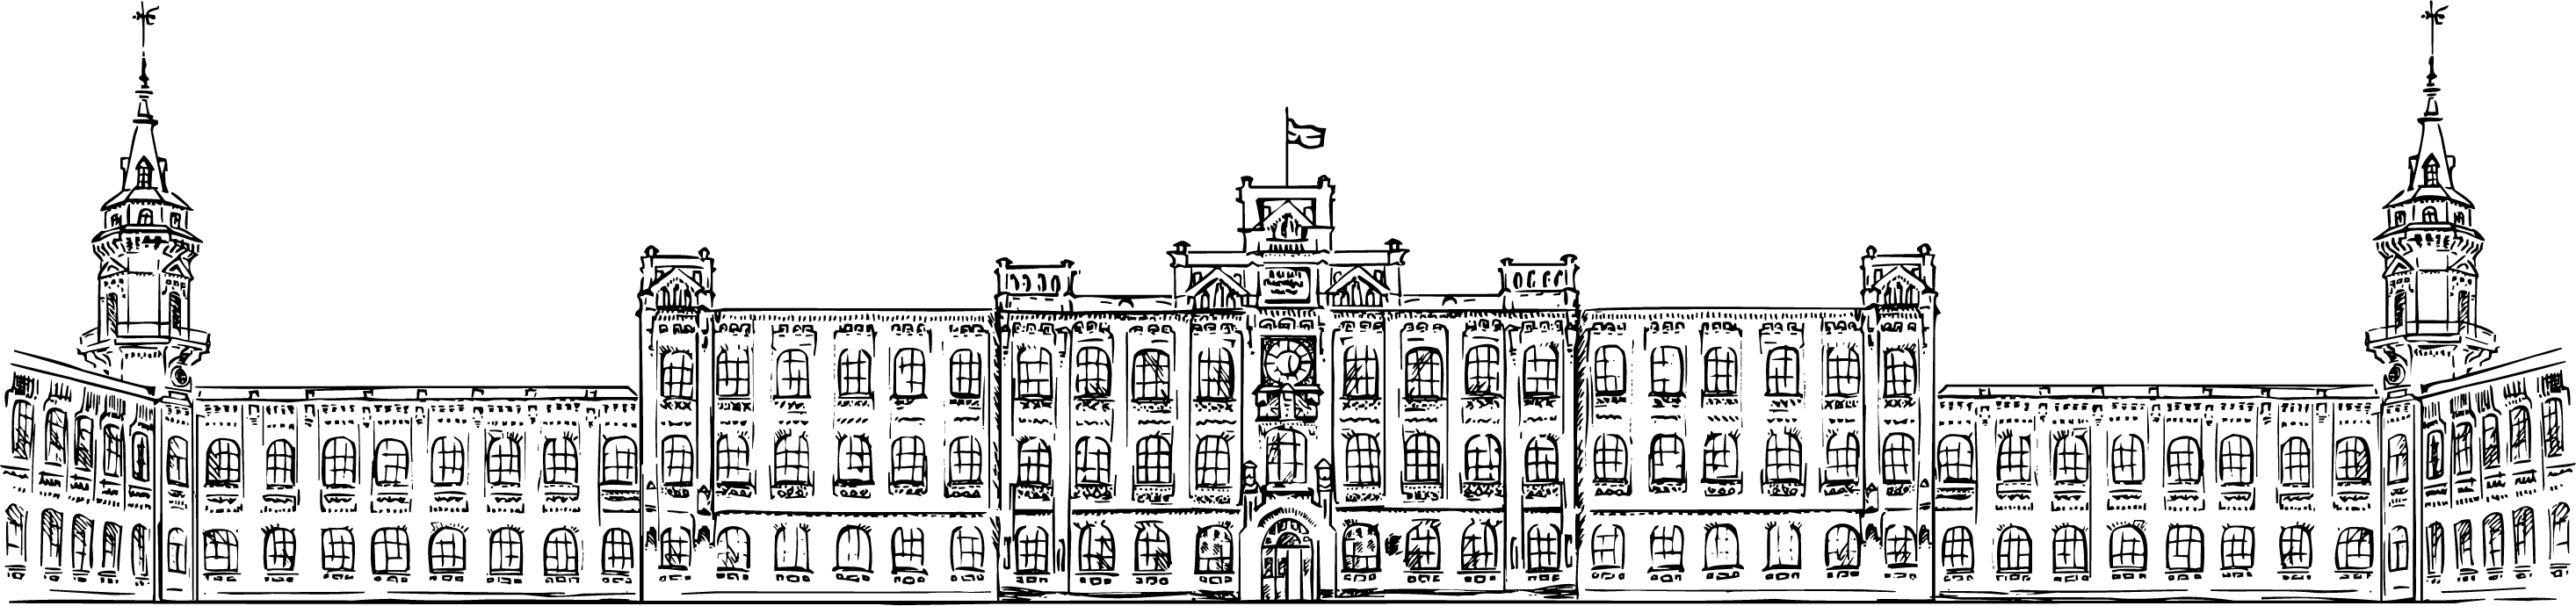
\includegraphics[width=0.7\textwidth]{../../../TITLES/letterhead.png}\end{center}

        \begin{center}
            \large Національний технічний університет України\\
            «Київський політехнічний інститут імені Ігоря Сікорського»\\[1em]
            Факультет інформатики та обчислювальної техніки\\
            Кафедра обчислювальної техніки
        \end{center}

        \vfill

        \begin{center}
            \textbf{\LARGE Інженерія програмного забезпечення}\\[2em]
            \textbf{\Large Практична робота №2}\\
            «Графічна нотація UML. Документування проекту»
        \end{center}

        \vfill

        \begin{flushright}
            Виконав: студент 2 курсу ФІОТ, гр. ІО-41\\
            \textit{Давидчук А.~М.}\\
            Залікова книжка № 4106\\[1em]
            Перевірив: \textit{Васильєва М.~Д.}
        \end{flushright}

        \vfill

        \begin{center}Київ --- 2025\end{center}

    \end{titlepage}

    % Основний документ:

    \setlength{\parindent}{0em}

    \textbf{\underline{Тема:}} «Графічна нотація UML. Документування проекту».
    
    \vspace{1em}

    \textbf{\underline{Мета:}} Ознайомитись з видами UML діаграм. Отримати базові навички з використання діаграми класів мови UML. Здобути навички використання засобів автоматизації UML-моделювання. Документування проекту за допомогою JavaDoc.

    \begin{center} \textbf{\Large Практична частина} \end{center}

    \setlength{\parindent}{1.5em}

    Мій номер залікової книги 4106, звідси $4106\text{ mod } 9 = 2$, і $4106\text{ mod } 5 = 1$. Звідси згідно переліку варіантів завдання, моя схема генералізації
    (наслідування):

    \begin{tcolorbox}[colback=gray!10, colframe=gray!50, arc=3pt, boxrule=0.5pt]
    If1 $\leftarrow$ If2; If1 $\leftarrow$ If3; Сl2 $\leftarrow$ Сl3
    \end{tcolorbox}

    і агрегації:

    \begin{tcolorbox}[colback=gray!10, colframe=gray!50, arc=3pt, boxrule=0.5pt]
    If1 $\leftarrow$ Cl2; Cl1 $\leftarrow$ Cl3; Cl1 $\leftarrow$ Cl1
    \end{tcolorbox}

    Звідси побудую UML-діаграму класів, яка відображає взаємозв'язки між трьома інтерфейсами (If1, If2, If3)
    та трьома класами (Cl1, Cl2, Cl3) згідно з моїм варіантом.
    Кожен інтерфейс містить методи \texttt{void meth1()}, \texttt{void meth2()}, \texttt{void meth3()}, а відповідний клас реалізує їх:

    \begin{figure}[h!]

        \renewcommand{\thefigure}{\arabic{figure}} % робимо "3.1", "3.2" і т.д.

        \centering
        % Підставляєте потрібний шлях та розмір зображення:
        \includegraphics[width=0.33\textwidth]{UMLDiagram.pdf}
        % Підпис (зазвичай під малюнком):
        \caption{UML-діаграма класів та інтерфейсів}
        % Мітка для посилань у тексті (\ref{fig:...})
        \label{fig1:UML_diagram}

    \end{figure}

    \newpage

    \setlength{\parindent}{0em}

    \textbf{\underline{Програмний код (\texttt{project1$\backslash$src$\backslash$lab2$\backslash$Main.java}):}}

    \begin{minted}{java}
package lab2;

/**
 * Клас Main призначений для тестування реалізованих класів і інтерфейсів.
 * Демонструє виклики методів і створення агрегованих зв'язків.
 * @author Artem Davydchuk
 * @version 1.0
 */

public class Main {
    /**
     * Точка входу до програми.
     * @param args аргументи командного рядка
     */
    public static void main(String[] args) {
        Cl1 c1 = new Cl1();
        Cl2 c2 = new Cl2();
        Cl3 c3 = new Cl3();

        // Агрегація
        c1.setPart2(c2);
        c1.setPart3(c3);
        c1.addChild(new Cl1());

        // Виклик методів
        c1.meth1();
        c2.meth2();
        c3.meth3();
    }
}
    \end{minted}

    \textbf{\underline{Код інтерфейсу If1 (\texttt{project1$\backslash$src$\backslash$lab2$\backslash$If1.java}):}}

    \begin{minted}{java}
package lab2;

/**
 * Базовий інтерфейс If1.
 * Містить три методи meth1(), meth2(), meth3().
 * Використовується як основа для If2 і If3.
 * @author Artem Davydchuk
 * @version 1.0
 */

public interface If1 {
    /**
     * Перший метод інтерфейсу If1.
     */
    void meth1();

    /**
     * Другий метод інтерфейсу If1.
     */
    void meth2();

    /**
     * Третій метод інтерфейсу If1.
     */
    void meth3();
}

    \end{minted}

    \textbf{\underline{Код інтерфейсу If2 (\texttt{project1$\backslash$src$\backslash$lab2$\backslash$If2.java}):}}

    \begin{minted}{java}
package lab2;

/**
 * Інтерфейс If2 успадковує If1.
 * Призначений для розширення функціональності базового інтерфейсу.
 * @author Artem Davydchuk
 * @version 1.0
 */

public interface If2 extends If1 {}
    \end{minted}

    \textbf{\underline{Код інтерфейсу If3 (\texttt{project1$\backslash$src$\backslash$lab2$\backslash$If3.java}):}}

    \begin{minted}{java}
package lab2;

/**
 * Інтерфейс If2 успадковує If1.
 * Призначений для розширення функціональності базового інтерфейсу.
 * @author Artem Davydchuk
 * @version 1.0
 */

public interface If3 extends If1 {}
    \end{minted}

    \textbf{\underline{Код класу Cl1 (\texttt{project1$\backslash$src$\backslash$lab2$\backslash$Cl1.java}):}}

    \begin{minted}{java}
package lab2;

import java.util.ArrayList;
import java.util.List;

/**
 * Клас Cl1 реалізує інтерфейс If1.
 * Містить поля-агрегації: об'єкти Cl2, Cl3 і список власних екземплярів (self-aggregation).
 * Кожен метод виводить у консоль своє ім'я для демонстрації викликів.
 * @author Artem Davydchuk
 * @version 1.0
 */
public class Cl1 implements If1 {
    /** Агрегований об'єкт типу Cl2.
    * @uml.aggregation */
    private Cl2 part2;

    /** Агрегований об'єкт типу Cl3.
     * @uml.aggregation */
    private Cl3 part3;

    /** Список підлеглих екземплярів Cl1 (самоагрегація). */

    private List<Cl1> children = new ArrayList<>();

    /**
     * Джерело опису: {@link If1#meth1()}.
     * {@inheritDoc}
     */
    @Override
    public void meth1() { System.out.println("Cl1: meth1"); }

    /**
     * Джерело опису: {@link If1#meth2()}.
     * {@inheritDoc}
     */
    @Override
    public void meth2() { System.out.println("Cl1: meth2"); }

    /**
     * Джерело опису: {@link If1#meth3()}.
     * {@inheritDoc}
     */
    @Override
    public void meth3() { System.out.println("Cl1: meth3"); }

    /**
     * Задає агрегований об'єкт типу Cl2.
     * @param p екземпляр Cl2
     */
    public void setPart2(Cl2 p) { this.part2 = p; }

    /**
     * Задає агрегований об'єкт типу Cl3.
     * @param p екземпляр Cl3
     */
    public void setPart3(Cl3 p) { this.part3 = p; }

    /**
     * Додає дочірній екземпляр Cl1 до списку.
     * @param child підлеглий об'єкт Cl1
     */
    public void addChild(Cl1 child) { this.children.add(child); }
}
    \end{minted}

    \textbf{\underline{Код класу Cl2 (\texttt{project1$\backslash$src$\backslash$lab2$\backslash$Cl2.java}):}}

    \begin{minted}{java}
package lab2;

/**
 * Клас Cl2 реалізує інтерфейс If2.
 * Реалізує всі методи базового інтерфейсу If1.
 * @author Artem Davydchuk
 * @version 1.0
 */

public class Cl2 implements If2 {
    /**
     * Джерело опису: {@link If1#meth1()}
     * (через {@link If2}).
     * {@inheritDoc}
     */
    @Override
    public void meth1() { System.out.println("Cl2: meth1"); }

    /**
     * Джерело опису: {@link If1#meth2()} (через {@link If2}).
     * {@inheritDoc}
     */
    @Override
    public void meth2() { System.out.println("Cl2: meth2"); }

    /**
     * Джерело опису: {@link If1#meth3()} (через {@link If2}).
     * {@inheritDoc}
     */
    @Override
    public void meth3() { System.out.println("Cl2: meth3"); }
}
    \end{minted}

    \textbf{\underline{Код класу Cl3 (\texttt{project1$\backslash$src$\backslash$lab2$\backslash$Cl3.java}):}}

    \begin{minted}{java}
package lab2;

/**
 * Клас Cl3 успадковує Cl2 та реалізує інтерфейс If3.
 * Реалізує всі методи з виведенням у консоль.
 * @author Artem Davydchuk
 * @version 1.0
 */

public class Cl3 extends Cl2 implements If3 {
    /**
     * Джерело опису: {@link Cl2#meth1()} (транзитивно з {@link If1#meth1()}).
     * {@inheritDoc}
     */
    @Override
    public void meth1() { System.out.println("Cl3: meth1"); }

    /**
     * Джерело опису: {@link Cl2#meth2()} (транзитивно з {@link If1#meth2()}).
     * {@inheritDoc}
     */
    @Override
    public void meth2() { System.out.println("Cl3: meth2"); }

    /**
     * Джерело опису: {@link Cl2#meth3()} (транзитивно з {@link If1#meth3()}).
     * {@inheritDoc}
     */
    @Override
    public void meth3() { System.out.println("Cl3: meth3"); }
}

    \end{minted}

    \textbf{\underline{Код збірки для Ant (\texttt{project1$\backslash$src$\backslash$build.xml}):}}

    \begin{minted}{xml}
<?xml version="1.0" encoding="UTF-8"?>
<project name="Lab2_Project1" default="all" basedir=".">

    <!-- ===== Налаштування шляхів ===== -->
    <property name="src.dir" value="src"/>
    <property name="build.dir" value="out"/>
    <property name="doc.dir" value="doc"/>
    <property name="main.class" value="lab2.Main"/>

    <!-- ===== 1. Компіляція Java-файлів ===== -->
    <target name="compile" description="Компіляція вихідних Java-файлів у теку out">
        <mkdir dir="${build.dir}"/>
        <javac
                includeantruntime="false"
                encoding="UTF-8"
                srcdir="${src.dir}"
                destdir="${build.dir}">
        </javac>
        <echo message="Компіляція завершена. Клас-файли збережено у '${build.dir}'."/>
    </target>

    <!-- ===== 2. Генерація JavaDoc ===== -->
    <target name="javadoc" description="Створення HTML-документації в каталозі doc">
        <mkdir dir="${doc.dir}"/>
        <!-- additionalparam="-Xdoclint:none -quiet" Щоб видалити попередження про конструктор класів -->
        <javadoc
                sourcepath="${src.dir}"
                destdir="${doc.dir}"
                encoding="UTF-8"
                docencoding="UTF-8"
                charset="UTF-8"
                author="true"
                version="true"
                use="true"
                additionalparam="-Xdoclint:none -quiet"
                windowtitle="JavaDoc – Lab2 Project1"
                doctitle="Документація до лабораторної роботи №2 – UML">
            <fileset dir="${src.dir}" includes="**/*.java"/>
        </javadoc>
        <echo message="JavaDoc успішно згенеровано у каталозі '${doc.dir}'."/>
    </target>

    <!-- ===== 3. Запуск програми ===== -->
    <target name="run" depends="compile" description="Запуск програми після компіляції">
        <echo message="Запуск програми ${main.class}..."/>
        <java classname="${main.class}" fork="true">
            <classpath>
                <pathelement path="${build.dir}"/>
            </classpath>
        </java>
        <echo message="Програму завершено."/>
    </target>

    <!-- ===== 4. Об'єднана команда ===== -->
    <target name="all" depends="compile, javadoc, run" description="Компіляція + JavaDoc + запуск">
        <echo message="Проєкт повністю зібрано, задокументовано та виконано."/>
    </target>

</project>
    \end{minted}

    Тут \texttt{build.xml} має такі команди збірки:

    \begin{minted}{text}
PS C:\Users\artem\OneDrive\Desktop\reps\university_roadmap\semestr3\software engineering\labs\lab2\project1> ant -p 
Buildfile: C:\Users\artem\OneDrive\Desktop\reps\university_roadmap\semestr3\software engineering\labs\lab2\project1\build.xml

Main targets:

 all      Комп?ляц?я + JavaDoc + запуск
 compile  Комп?ляц?я вих?дних Java-файл?в у теку out
 javadoc  Створення HTML-документац?ї в каталоз? doc
 run      Запуск програми п?сля комп?ляц?ї
    \end{minted}

    Виконуємо збірку (команда \texttt{all} є default-командою):

    \begin{minted}{text}
PS C:\Users\artem\OneDrive\Desktop\reps\university_roadmap\semestr3\software engineering\labs\lab2\project1> ant 
Buildfile: C:\Users\artem\OneDrive\Desktop\reps\university_roadmap\semestr3\software engineering\labs\lab2\project1\build.xml

compile:
     [echo] Комп?ляц?я завершена. Клас-файли збережено у 'out'.

javadoc:
  [javadoc] Generating Javadoc
  [javadoc] Javadoc execution
     [echo] JavaDoc усп?шно згенеровано у каталоз? 'doc'.

run:
     [echo] Запуск програми lab2.Main...
     [java] Cl1: meth1
     [java] Cl2: meth2
     [java] Cl3: meth3
     [echo] Програму завершено.

all:
     [echo] Проєкт повн?стю з?брано, задокументовано та виконано.

BUILD SUCCESSFUL
Total time: 1 second
    \end{minted}

    Результат вікдриття файлу документації \texttt{index.html} (у браузері):

    \begin{figure}[h!]

        \renewcommand{\thefigure}{\arabic{figure}} % робимо "3.1", "3.2" і т.д.

        \centering
        % Підставляєте потрібний шлях та розмір зображення:
        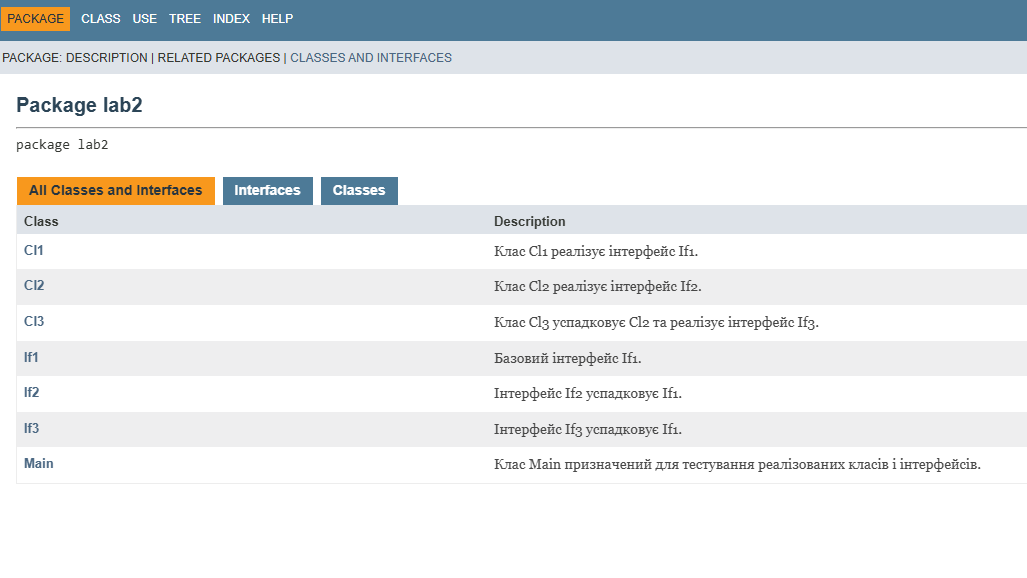
\includegraphics[width=0.5\textwidth]{docres1.png}
        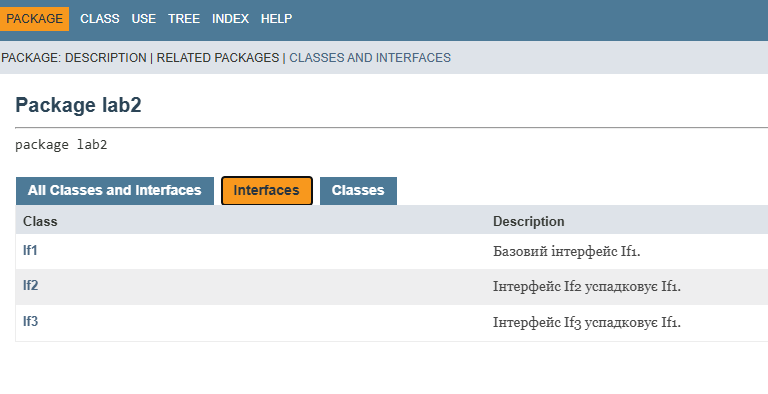
\includegraphics[width=0.5\textwidth]{docres2.png}
        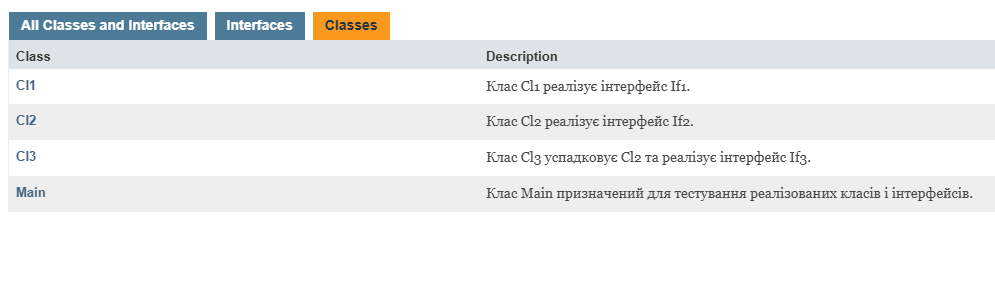
\includegraphics[width=0.5\textwidth]{docres3.png}
        % Підпис (зазвичай під малюнком):
        \caption{Сторінка документації коду у браузері}
        % Мітка для посилань у тексті (\ref{fig:...})
        \label{fig2:doc}

    \end{figure}

    \newpage

    Далі за допомогою \texttt{PlainUML Plugin} згенерую UML-діаграму на основі всього робочого \texttt{*.java} коду:

     \begin{figure}[h!]

        \renewcommand{\thefigure}{\arabic{figure}} % робимо "3.1", "3.2" і т.д.

        \centering
        % Підставляєте потрібний шлях та розмір зображення:
        \includegraphics[width=0.5\textwidth]{javaUMLgenerated.pdf}
        % Підпис (зазвичай під малюнком):
        \caption{Згенерована UML-діаграма на основі коду}
        % Мітка для посилань у тексті (\ref{fig:...})
        \label{fig3:umlGenerated}

    \end{figure}

    \setlength{\parindent}{1.5em}

    Згенерована UML-діаграма з коду пакета \texttt{lab2} повністю відповідає розробленій вручну за складом класів та інтерфейсів. 
    Різниця полягає у рівні деталізації: автоматично створена діаграма не дублює методи інтерфейсів у класах-реалізаціях, 
    а зв'язки типу агрегації (\texttt{If1$\leftarrow$Cl2}, \texttt{Cl1$\leftarrow$Cl3}, \texttt{Cl1$\leftarrow$Cl1}) відображено як звичайні асоціації, 
    оскільки їх тип не може бути однозначно визначений з коду. Таким чином, обидві діаграми еквівалентні за структурою, відмінності мають лише візуальний характер.

    \setlength{\parindent}{0em}

    \textbf{\underline{Висновок:}} У ході роботи було побудовано базову UML-діаграму класів із трьома інтерфейсами та трьома класами, 
реалізовано зв’язки генералізації та агрегації згідно з індивідуальним варіантом, 
створено відповідний вихідний код мовою~Java, згенеровано документацію~JavaDoc 
та налаштовано сценарій автоматизації складання проєкту у~\texttt{build.xml}. 
За допомогою засобів генерації UML-діаграм із вихідного коду перевірено відповідність UML-діаграми моделі програми. 
Згенерована діаграма повністю підтвердила коректність реалізації зв’язків та структури вручну створеної UML-діаграми.

\end{document}